The previous paragraph noted the importance of absolute and conditional independence relationships in simplifying probabilistic representation.
This section introduces a systematic way to represent such relationships in the form of \textbf{Bayesian networks}.
We define the syntax and semantics of these networks and show how they can be used to capture uncertain knowledge. \vspace{7pt}

A Bayesian network is a simple graphical notation for conditional independence assertions and hence for a compact specification of full joint distribution.
The Bayesian network's syntax is composed by:
\begin{enumerate}
    \item Each node corresponds to a random variable.
    \item A set of directed links or arrows connects pairs of nodes.
    \item Each node $X_i$ has a conditional probability distribution $\mathbf{P}(X_i|Parents(X_i))$, that quantifies the effect of the parents on the node.
\end{enumerate}
\begin{example}
    i.e. Topology of network encodes conditional independence assertions: \vspace{3.5pt}
    \begin{center}
        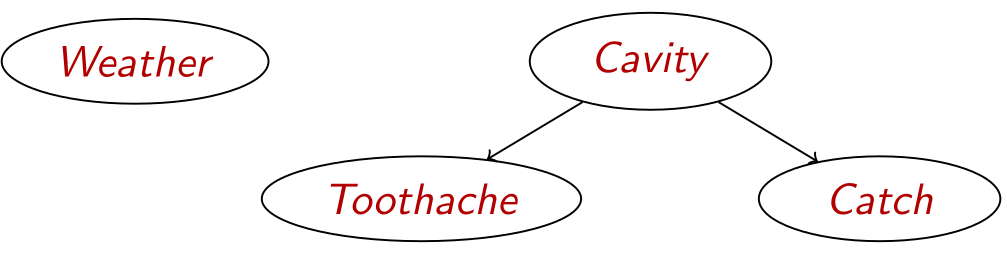
\includegraphics[width=0.6\textwidth]{img/img2.png}
    \end{center} \vspace{3.5pt}
    \begin{itemize}
        \renewcommand{\labelitemi}{-}
        \item Weather is independent of the other variables\footnote{Formally, the absolute or conditional independence is indicated by the absence of a link between nodes.}.
        \item Toothache and Catch are conditionally independent given Cavity\footnote{The intuitive meaning of an arrow is typically that X has a direct influnce on Y, which suggests that causes should be parents of effects.}.
    \end{itemize}
\end{example}
\begin{example}
    i.e. I'm at work, neighbor John calls to say my alarm is ringing, but neighbor Mary doesn't call. Sometimes it's set off by minor earthquakes. Is there a burglar? \vspace{3.5pt}

    The random variables are: \it Burglar, Earthquake, Alarm, MaryCalls, JohnCalls \footnote{The network topology reflects \textbf{causal} knowledge, from the causes nodes we define the effects nodes.}\footnote{For each node the conditional distribution are shown as a \textbf{conditional probability table}, or simply CPT.}\footnote{Let's take a look at the tables. In this network we are talking about joint distribution, not full joint distribution. Simply, the full joint distribution about boolean random variables can be computed by $1-P(a)$.}. \vspace{3.5pt}
    \begin{center}
        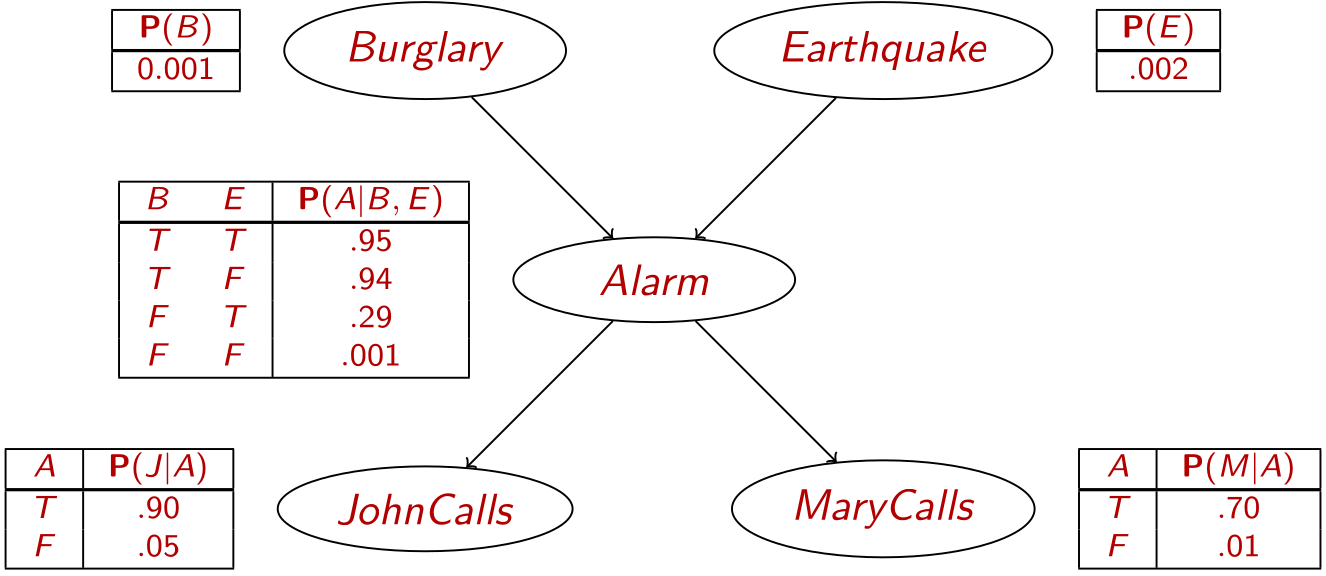
\includegraphics[width=0.75\textwidth]{img/img3.png} \vspace{3.5pt}
    \end{center}
\end{example}

We begin the discussion with a simple toy example, the \textit{student network}.
\begin{example}
    i.e. A student's grade depends on intelligence and on the difficulty of the course.
    SAT scores are correlated with intelligence. A professor writes recommendation letters by only looking at grades. \vspace{3.5pt}

    In this case, our probability space is composed by five relevant random variables: \textit{Difficulty (D)}, \textit{Intelligence (I)}, \textit{SAT score (S)}, \textit{Grade (G)} and \textit{Letter (L)}. \vspace{3.5pt}
    \begin{center}
        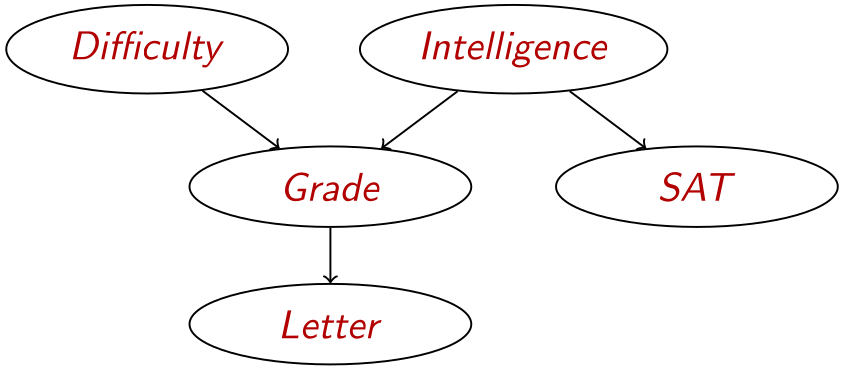
\includegraphics[width=0.5\textwidth]{img/img4.png}
    \end{center} \vspace{3.5pt}
    Consider a particular student, George, that he would like to reason using the student network. We might ask how likely George is to get a strong recommendation from his professor in Analysis.
    Knowing nothing else about George and his grade, this probability is around the $50$ percent. \vspace{3.5pt}

    We now find out that George is not so intelligent. The probability that he gets a strong letter from the professor goes down to 39. We now further discover that Analysis is an easy class.
    The probability that George receive a strong letter is now about 51 percent. \vspace{3.5pt}

    Queries and answers such as this, where we predict the behaviors from causes to effects, are called \textbf{causal reasoning} or \textbf{prediction}\footnote{It reflects the causal direction, from the parent nodes we are just defining which is their influence on their children.}. \vspace{3.5pt}

    Now, assume a recruiter, trying to hire George based on our previous model. By a prior probability, the recruiter believes that George is 30 percent likely to be intelligent. 
    He obtains George's grade record for the class Analysis and sees that George received a low score in that class. His probability that George has high intelligence goes down,
    about 7.9 percent. We note that the probability that the class is a difficult one also goes up, from 40 percent to 62.9 percent. Now, consider that the recruiter lost George's trascript of records, and has only the recommendation letter from George's professor in Analysis, which is weak.
    The probability that George has high intelligence still goes down, but only to 14 percent. Note that if the recruiter has both the grade and the letter, we have the same probability
    as if he had only the grade. \vspace{3.5pt}

    Queries such as this, where we reason from effects to causes, are named \textbf{evidential reasoning} or \textbf{explanation}\footnote{In this case, we are not reasoning from top to bottom, but instead from bottom to top.}. \vspace{3.5pt}

    Finally, George submits his high SAT score to the recruiter. The probability that George has high intelligence goes up dramatically, from 7.9 percent to 57.8 percent. Intuitively, the reason that the SAT score 
    outweights the poor grade is that a student with low intelligence are unlikely to get good scores on their SAT, whereas students with high intelligence can still get C grades in hard class.
    Indeed, we see that the probability that Analysis is a difficult one goes up from 62.9 percent to 76 percent. \vspace{3.5pt} 

    This last pattern is a interesting one. The information about SAT score told us other informations about the student's intelligence, which, in conjuction with the student's grade, gave us some clues about the difficulty of the course. Let examine this pattern in probabilistic terms. \vspace{3.5pt}

    We are saying \vspace{3.5pt}

    $P_s(i^1|g^3) = 0.079$ \vspace{3.5pt}

    On the other hand, if we consider that Analysis is a hard class, we have \vspace{3.5pt}

    $P_s(i^1|d^1, g^3) = 0.11$ \vspace{3.5pt} 

    Here, we are partially explaining why George has got a poor grade. By the way, taking a more tricky example, for instance George got a middle grade in Analysis, we have that \vspace{3.5pt}

    $P_s(i^1|g^2) = 0.175$ \vspace{3.5pt}

    Also if Analysis is a hard class, we get \vspace{3.5pt} 

    $P_s(i^1|d^1, g^2) = 0.34$ \vspace{3.5pt} 

    In effect, we have justified the poor grade via the difficulty of the class. Explaining away is an instance of a general pattern called \textbf{intercasual reasoning},
    where different causes of the same effect, so they are parents of the effect node, can interact.     
\end{example}
\textbf{Compactness} \vspace{3.5pt}

A Bayesian network can often be more \textit{compact} than the full joint distribution. The \textbf{compactness} of a Bayesian network is a property that makes easy to handle
domain with many random variables. \vspace{3.5pt}

At the same time, a Bayesian network grows \textit{linearly}, instead of an \textit{exponential} growth by full joint distribution. Assuming a domain composed by $\mathbf{n}$ Boolean
variables, where each of them is associated with a CPT \textit{(Conditional Probability Table)}\footnote{A CPT for a Boolean variable $\mathbf{X_i}$ with $\mathbf{k}$ parents, has $\mathbf{2^k}$
rows for the combinations of parents values and usually is defined only the True case; the negative case, however $X_i = False$, can be simply computed by the third probability axiom $\mathbf{1 - p}$.}.
If each variable has no more then $\mathbf{k}$ parents, the complete network requires $O(n \times 2^k)$ numbers, as we already know to complete the full joint distribution are necessary
$O(2^n)$.
\begin{example}
    i.e. Comparison of parameters required from the previously example between Bayesian network and full joint distribution. \vspace{3.5pt}

    For the burglar network: \vspace{3.5pt}

    $1 + 1 + 4 + 2 + 2 = 10$ numbers required by the Bayesian network \vspace{3.5pt}

    $2^5 - 1 = 47$ numbers required by the full joint distribution
\end{example}
\textbf{Global semantics} \vspace{3.5pt}

A Bayesian network is a directed acyclic graph with some numeric parameters attached to each node. One way to define what the network means is to define the way in which 
it rapresents a full joint distribution. 
\begin{definition}
    \textbf{Global semantics} defines the full joint distribution as the product of the local conditional distributions:
    \begin{center}
        $P(x_1, ..., x_n) = \prod_{i = 1}^{n} P(x_i|parents(X_i))$
    \end{center}
\end{definition}
\begin{example}
    i.e. 
    
    $P(j, m, a, \neg b, \neg e) \\
    = P(j|a)P(m|a)P(a|\neg b \wedge \neg e)P(\neg b)P(\neg e) \\
    = 0.9 \times 0.7 \times 0.001 \times 0.999 \times 0.998 = 0.000628$
\end{example}
\textbf{Flow of influence} \vspace{3.5pt}

Until now, we used the intuition that edges represent direct dependence. For instance, we said that the letter recommendation from the professor depends only on the student's grade;
this state was encoded by the fact that there is an exit edge from \textit{G} that arrive to \textit{L}. This intuition is \textbf{not} always true. \vspace{3.5pt}

The aim of this section is to understand when we can guarantee independence between random variables. First of all, we begin with a simple case analysis: we try to understand
when a variable \textbf{X} can influence \textbf{Y} given \textbf{Z}. \vspace{3.5pt}

\textbf{Direct connection}. This is the simple case, when X and Y are directly connected via an edge. If X and Y are directly connected, we can always get examples where they 
influence each other, regardless of \textbf{Z}. \vspace{3.5pt}

\textbf{Indirect connection}. Now  we are considering the more complicated case when X and Y are not directly connected, but there is a trail between them. There are four cases
where X and Y are connected via Z. \vspace{3.5pt}
\begin{center}
    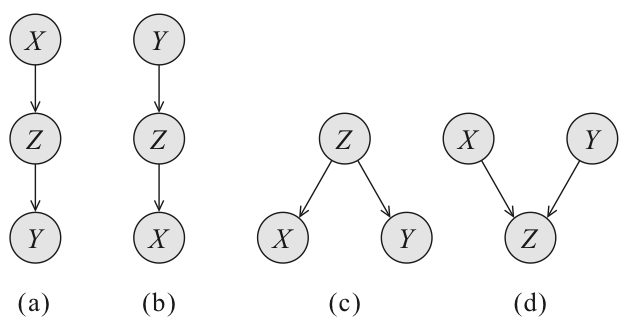
\includegraphics[width=0.6\textwidth]{img/img5.png}
\end{center} \vspace{3.5pt}
The first two correspond to causal chains, the third to a common cause, and the last one to a common effect.

\textbf{(a) Causal trail}. We have a chain like $X \rightarrow Z \rightarrow Y$. X cannot influence Y via Z if Z is observed.

\textbf{(b) Effect trail}. Now we have the same trail but in the opposite direction, so  $Y \rightarrow Z \rightarrow X$. Another time, Y cannot influence X via Z if Z is observed.

\textbf{(c) Common cause}. This type of trail defines the same grade of independence as before. If Z is observed then neither X or Y can influence each other. 

\textbf{(d) Common effect}. In the previously cases, we see a common pattern: if Z is observed then neither X or Y can influence each other. By the way, this kind of trail, 
$X \rightarrow Z \leftarrow Y$, has a new behavior. If Z is not observed influence cannot flow along the trail. So if Z is observed X and Y are independent. In the student example
we analyzed this case, which we called \textit{intercausal reasoning}; we showed that the probability that student has high intelligence goes down when we observe that his grade is 
a poor score, but then goes up when we observe that the class is a hard one. Let us consider a variant of the same case. Assume that we do not observe the student's grade, but we observed
that he received an awful recommendation letter. Intuitively, the same phenomenon happens. The weak letter told us that he received a low grade, and it is sufficient to 
correlate Intelligence and Difficulty.  
\begin{definition}
    If influence can flow from X to Y via Z, the trail $X \longleftrightarrow Z \longleftrightarrow Y$ is \textbf{active}.
\end{definition}
If we consider a longer trail $X_1 \rightarrow \dots \rightarrow X_n$, the first variable $X_1$ can influence the last variable $X_n$, if influence can flow through every single node of the trail.
This will be true if and only if every two-edge trail $X_{i-1} \longleftrightarrow X_i \longleftrightarrow X_{i+1}$ along the trail allows influence to flow.
\begin{definition}
    Let \textbf{Z} be a subset of observed variables. The trail $X_{i-1} \longleftrightarrow X_i \longleftrightarrow X_{i+1}$ is \textbf{active given} Z if
    \begin{itemize}
        \renewcommand{\labelitemi}{-}
        \item $\forall X_{i-1} \rightarrow X_i \leftarrow X_{i+1}$, $X_i$ or one of its descendants are in Z\footnote{The trail reported is the common effect case.}
        \item no other node along the trail is in Z
    \end{itemize}
\end{definition}
However, inside the Bayesian network literacy there is another important notion, named \textbf{d-separation}.
\begin{definition}
    Two sets of nodes \textbf{X}, \textbf{Y} are d-separated given Z if there is no active trail between any $X \in \mathbf{X}$ and $Y \in \mathbf{Y}$ given \textbf{Z}.
\end{definition}
It's possible to summarize few steps to follow to determine if X and Y are independent given Z:
\begin{enumerate}
    \item Mark all nodes in Z or having descendants in Z.
    \item Traverse the graph from X to Y, stopping if we get to a \textbf{blocked} node\footnote{A node is blocked if that node is the middle of an unmarked v-structure \textit{(common effect case)}, or belongs to Z \textit{(cannot be both).}}.
    \item If we can't reach Y, then X and Y are independent.
\end{enumerate}
Another aspects about independence are introduces by the meaning of \textbf{local semantics} and \textbf{Markov blanket}.
\begin{definition}
    \textbf{Local semantics} define that each node is conditionally independent of its \textbf{non-descendants} given its parents\footnote{Here, we are considering the parents of the first node, not the parents of non-descendants.}. 
\end{definition}
\begin{definition}
    Each node is conditionlly independent of all the others nodes given its \textbf{Markov blanket}: so its parents, children and children's parents.
\end{definition}